%
\section{Hardware specification}
\label{sec:hw-specs}
The first step for system design is the \gls{hw} specification. This can be pictured as a block diagram, this block diagram was already shown and mentioned in section \ref{sec:hardw-arch} on Fig.~\ref{fig:hw-arch}.

\subsection{Architecture}
\label{sec:arch}
Although that in the analysis phase an overview of the \gls{hw} architecture was conceptualized, in this section, a more specific \gls{hw} architecture is illustrated, using a block-diagram.

As it can be seen in Fig.~\ref{fig:hw-arch-complete}, the \texttt{Raspberry Pi} is the main controller and it is powered by the \texttt{Power Supply} through \texttt{USB-C}. 
The \texttt{Power Supply} also supplies via \texttt{Micro-USB} the \texttt{LCD Display} control board and the \texttt{Fragrance Diffusion Actuator}.
The \texttt{LCD Display} board connects to its board through \texttt{50-pin \gls{ttl}} and the board connects to the \texttt{Raspberry Pi} through \texttt{\gls{hdmi}}.
The \texttt{Speakers} also connect to the \texttt{LCD Display} board through \texttt{JST PH2.0}.
Beyond being powered up, the \texttt{Fragrance Diffusion Actuator} also connects to the \texttt{Raspberry Pi} through the \texttt{\gls{gpio}}.
What also connects to the \texttt{Raspberry Pi} through \texttt{\gls{gpio}} are the \texttt{Motion Detection} sensors.
Lastly, the \texttt{Camera} connects through \texttt{\gls{csi}} to the \texttt{Raspberry Pi}.
%
\begin{figure}[htb!]
\centering
    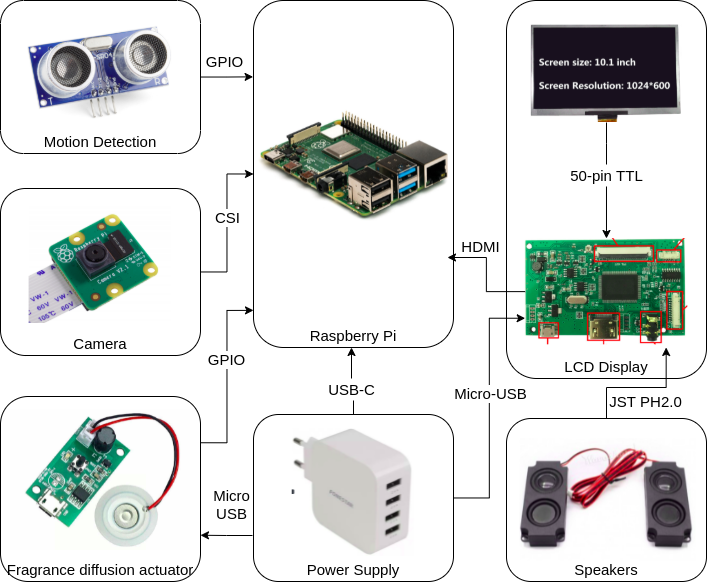
\includegraphics[width=0.8\columnwidth]{./img/hw-arch-complete.png}
  \caption{\gls{hw} architecture Block Diagram}%
\label{fig:hw-arch-complete}
\end{figure}

\subsection{Main Controller}
\label{sec:main-contr}

The main controller was also previously mentioned because it makes part of one of the requirements of this project: use the Raspberry Pi 4B (Fig.~\ref{fig:raspberri}).
This \gls{soc} has several of specifications~\cite{rasp-specs}:
%
\begin{item-c}
\item \emph{Processor}: it has the Broadcom BCM2711 processor, quad-core Cortex-A72 (ARM v8) 64-bit with 1.5GHz;
%
\item \emph{Memory}: this model has 4GB LPDDR4 with on-die ECC;
%
\item \emph{Connectivity}: it has a 2.4 GHz and 5.0 GHz IEEE 802.11b/g/n/ac wireless LAN, Bluetooth 5.0 with low energy, one Gigabit Ethernet port, four USB ports in which two are 3.0 and another two are 2.0;
%
\item \emph{GPIO}: it has a standard 40-pin \gls{gpio} header that is fully backwards-compatible with previous boards;
%
\item \emph{Video and Sound}: it has two \gls{hdmi} ports that support up to 4kp60, a 2-lane MIPI DSI display port, a 2-lane MIPI CSI camera port and a 4-pole stereo audio and composite video port;
%
\item \emph{Multimedia}: H.265 (4Kp60 decode), H.264(1080p60 decode and 1080p30 encode) and OpenGL ES 3.0 graphics;
%
\item \emph{SD card support}: Micro SD card slot for loading operating system and data storage;
%
\item \emph{Input power}: it has 5V \gls{dc} via USB-C connector (minimum 3A), a 5V \gls{dc} via \gls{gpio} header (minimum 3A) and \gls{poe} - enabled (requires separate \gls{poe} HAT);
%
\item \emph{Environment}: it has a range of operation between 0ºC and 50ºC.
\end{item-c}
%
\begin{figure}[htb!]
\centering
    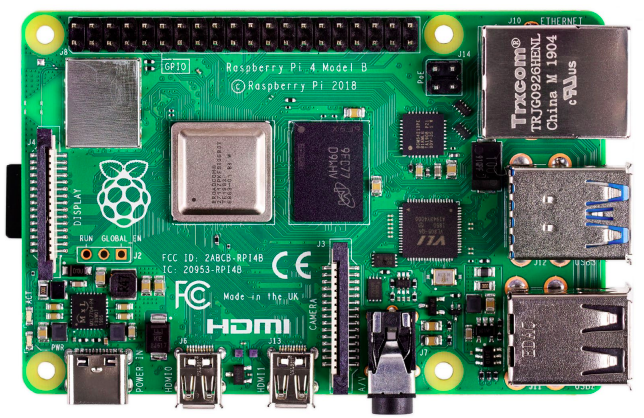
\includegraphics[width=0.6\columnwidth]{./img/raspberry.png}
  \caption{Raspberry Pi model 4B}%
\label{fig:raspberri}
\end{figure}

\subsubsection{SD Card}

Since this Raspberry supports SD Card, it will be used a micro SD Card with 16 GB that will store everything that is necessary to run the system and handle it.

\subsection{Motion Detection}
\label{sec:motion-detec}

For the motion detection, it was already mentioned in section \ref{sec:motion-detection} that the best option is to use an ultrasonic sensor. Thus, the sensor that has been chosen is the \texttt{HC-SR04 Ultrasonic Sensor}. This sensor has the following specifications~\cite{sensor}:
%
\begin{item-c}
\item \emph{Operating Voltage}: 5V \gls{dc};
\item \emph{Operating Current}: 15 \gls{ma};
\item \emph{Operating Frequency}: 40 KHz;
\item \emph{Maximum Range}: 4 meters;
\item \emph{Minimum Range}: 2 centimeters;
\item \emph{Ranging Accuracy}: 3 millimeters;
\item \emph{Measuring Angle}: 15 degrees;
\item \emph{Trigger Input Signal}: 10 microseconds \gls{ttl} pulse;
\item \emph{Dimension}: 45 x 20 x 15 millimeters.
\end{item-c}

\subsubsection{Sensor Pinout}

In Fig.~\ref{fig:sensor-pinout} is described the sensor pinout and each pin works as follows~\cite{sensor}:
%
\begin{enum-c}
\item is the power supply for HC-SR04 Ultrasonic distance sensor which we connect to a 5V supply (for example, 5V pin on Raspberry);
\item pin that is used to trigger the ultrasonic sound pulses;
\item pin that produces a pulse when the reflected signal is received. The length of the pulse is proportional to the time it took for the transmitted signal to be detected.
\item pin that should be connected to the ground (for example, GND pin of the Raspberry).
\end{enum-c}
%
\begin{figure}[htb!]
\centering
    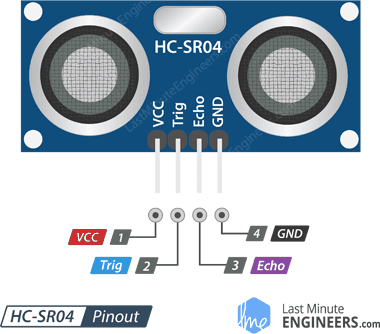
\includegraphics[width=0.4\columnwidth]{./img/sensor-pinout.png}
  \caption{HC-SR04 Pinout (withdrawn from \cite{sensor})}%
\label{fig:sensor-pinout}
\end{figure}

For this project it will be used three sensors, one placed on the bottom, another on the middle and another one on the top of the machine. 
With this setup, it can be avoided some perturbations like an animal walking in front of the machine (only the bottom sensor will detect). The disposition of the middle and top sensors can't be too high, because of short people, for example.

%\subsubsection{How does it work}
%On Fig.\ref{fig:sensor-behavior-ex} is an example on how does the sensor works.
%
%\begin{figure}[htb!]
%\centering
%    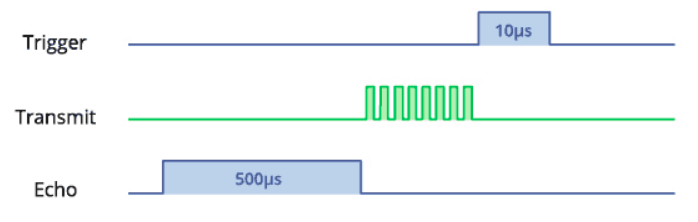
\includegraphics[width=0.6\columnwidth]{./img/sensor-behaviour-ex.png}
%  \caption{HC-SR04 behavior example (withdrawn from %\cite{sensor})}%
%\label{fig:sensor-behavior-ex}
%\end{figure}

%It all starts, when a pulse of at least 10 microseconds in duration is applied to the Trigger pin. In response to that, the sensor transmits a sonic burst of eight pulses at 40 KHz. This 8-pulse pattern makes the "ultrasonic signature" from the device unique, allowing the receiver to differentiate the transmitted pattern from the ambient ultrasonic noise~\cite{sensor}.

%The eight ultrasonic pulses travel through the air away from the transmitter. Meanwhile the Echo pin goes \texttt{HIGH} to start forming the beginning of the echo-back signal.
%In case, If those pulses are not reflected back then the Echo signal will timeout after 38 milliseconds and return \texttt{LOW}. Thus a 38 milliseconds pulse indicates no obstruction within the range of the sensor~\cite{sensor}.

%After the echo pin return low, it can be verified the distance of the obstacle to the sensor through some mathematics calculations.
%It is known that in this case \texttt{distance = time * speed}, being speed the speed of sound and time the time of the pulse.

\subsection{Fragrance Diffusion Actuator}

The chosen fragrance diffusion actuator is in Fig.~\ref{fig:fragrance-module} and has the following specifications~\cite{fragrance-module}:

It has an operating voltage of \texttt{5V \gls{dc}} and an operating current of \texttt{300 \gls{ma}}. The operating power is \texttt{2 Watt}. It has a fixed frequency single-chip microcomputer with a frequency of \texttt{108 KHz}. The dimensions of the board of the module are \texttt{35 * 20 * 17 millimeters}.
It has a \texttt{strong versatility}, large amount of fog, \texttt{stable performance}, the chip has an automatic timing shutdown function (4 hours of continuous work will automatically shut down protection, to turn on again, press the power on again). The 5V USB power supply mode, can be powered by MICRO charging cable.
The net diameter of the atomized steel sheet is 16 millimeters, the outer diameter of the silicone ring is 20 millimeters, and the wire length is 8 centimeters.
%
\begin{figure}[htb!]
\centering
    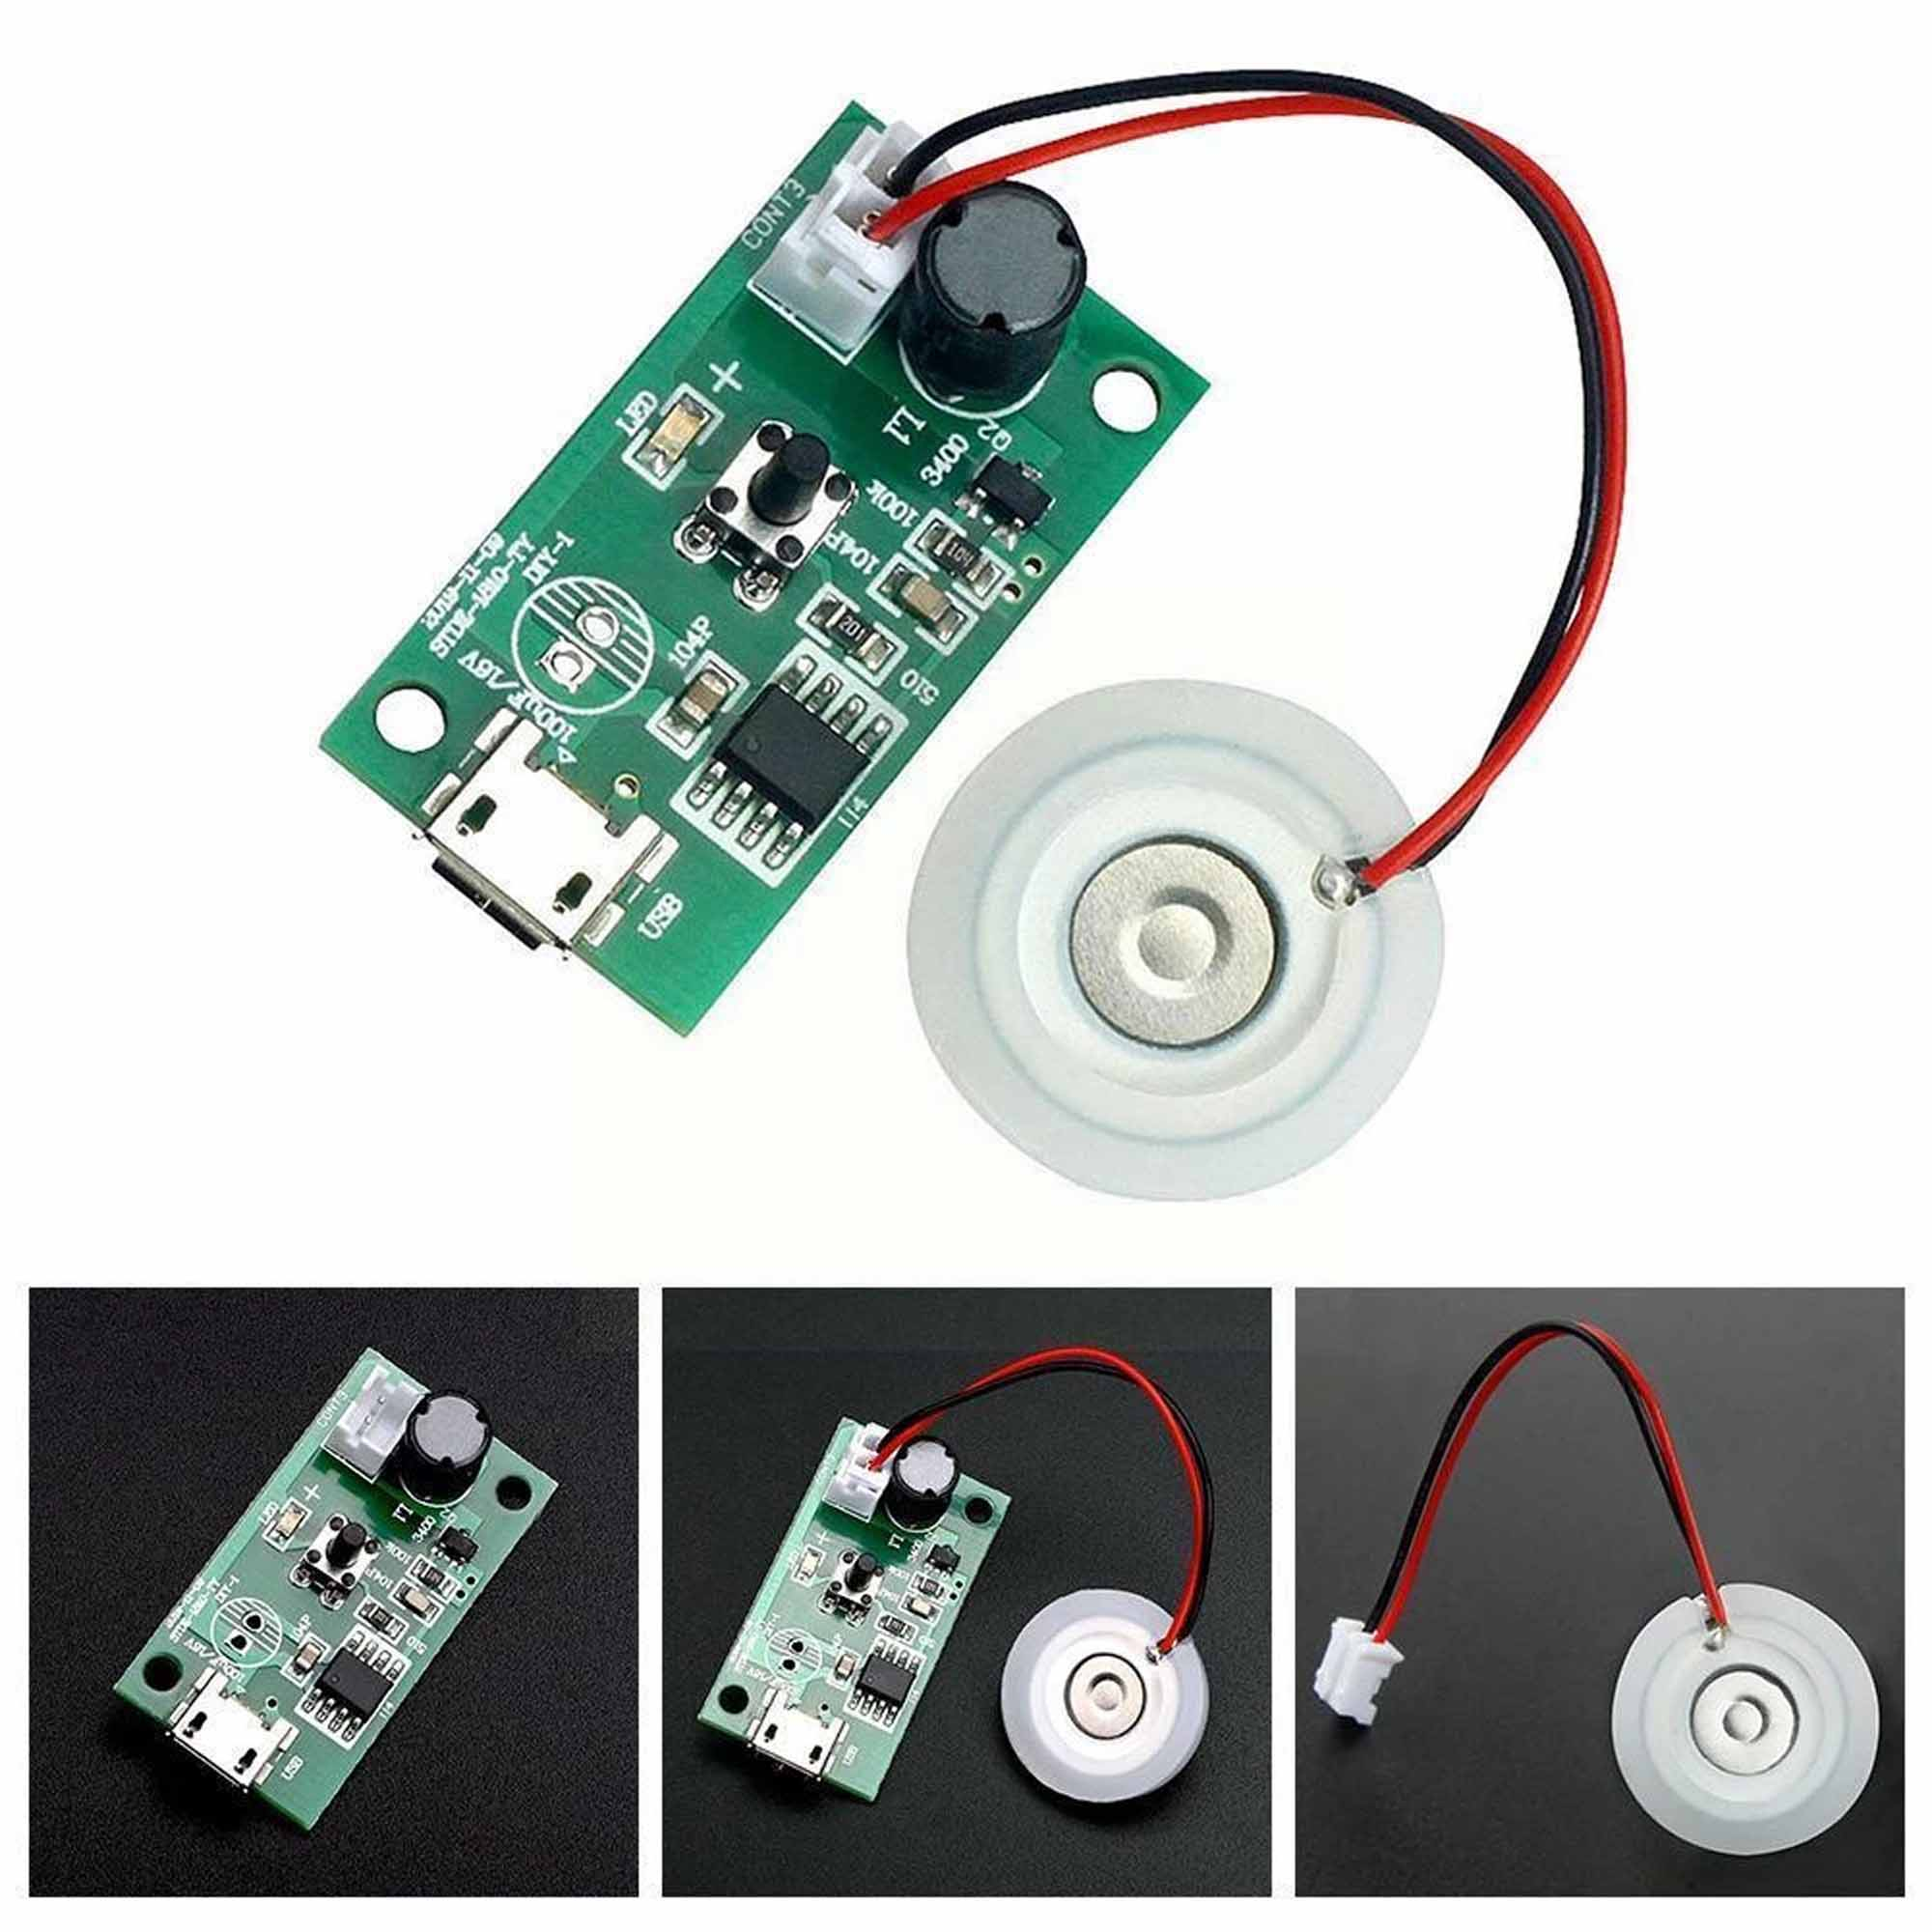
\includegraphics[width=0.5\columnwidth]{./img/fragrance-module.jpg}
  \caption{Fragrance module (withdrawn from \cite{fragrance-module})}%
\label{fig:fragrance-module}
\end{figure}


\subsection{Camera}
The camera to use in this project needs to be compatible with the board in use, in this case, the Raspberry Pi.
Thus the camera module that is used is the \texttt{Raspberry Pi Camera Module V2} (Fig.~\ref{fig:camera-module}).
%
\begin{figure}[htb!]
\centering
    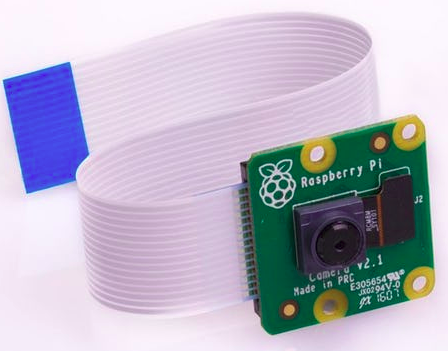
\includegraphics[width=0.4\columnwidth]{./img/camera-module.png}
  \caption{Camera module (withdrawn from \cite{camera-module})}%
\label{fig:camera-module}
\end{figure}

This camera module has a \texttt{Sony IMX219 8-megapixel sensor} and can be used to take high-definition video, as well as stills photographs. It supports 1080p30, 720p60 and VGA90 video modes, as well as still capture. It attaches via a 15 centimeters ribbon cable to the \gls{csi} port on the Raspberry Pi. The camera works with all models of Raspberry Pi 1, 2, 3 and 4. It can be accessed through the MMAL and V4L APIs, and there are numerous third-party libraries built for it, including the Picamera Python library.~\cite{camera-module}.

\subsection{LCD Display}

In Fig.~\ref{fig:screen} is the display that is used in this project. One advantage on this display is that it has \texttt{audio drivers}, which means that it is only necessary to plug a speaker and the board can handle the rest. It is also important to refer that the display isn't touch because there is no need to it and also this was the chosen one because it was the bigger and best on market considering quality and price.

As it can be seen, the display has \texttt{10.1 inches} and it is supplied with \texttt{5V \gls{dc}} and with a current of \texttt{2 A} via a micro USB port.
Fig.~\ref{fig:screen-interfaces} show all the interfaces that the board module of the display provides. That was also one more reason for the choice of this display: it has an \texttt{\gls{hdmi} interface} to connect to the Raspberry, the \texttt{50Pin TTL Screen Interface} that will connect to the display and two options to plug audio - the \texttt{Speaker Interface} and the \texttt{3.5mm audio interface}.
%
\begin{figure}[htb!]
\centering
    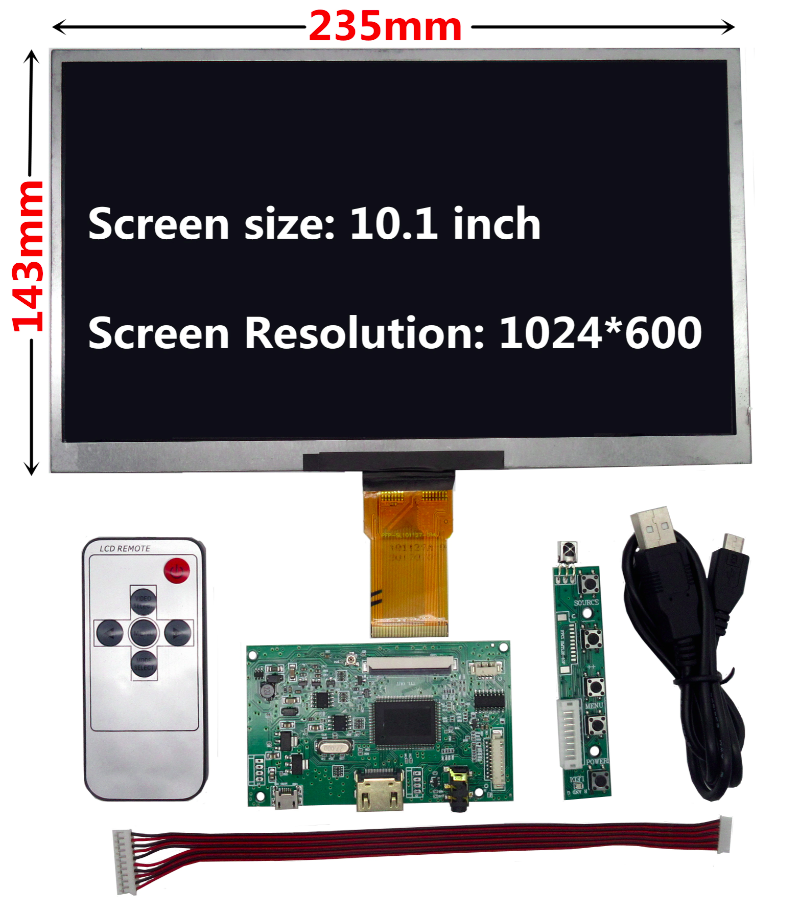
\includegraphics[width=0.4\columnwidth]{./img/screen.png}
  \caption{Display (withdrawn from \cite{screen})}%
\label{fig:screen}
\end{figure}
%
\begin{figure}[htb!]
\centering
    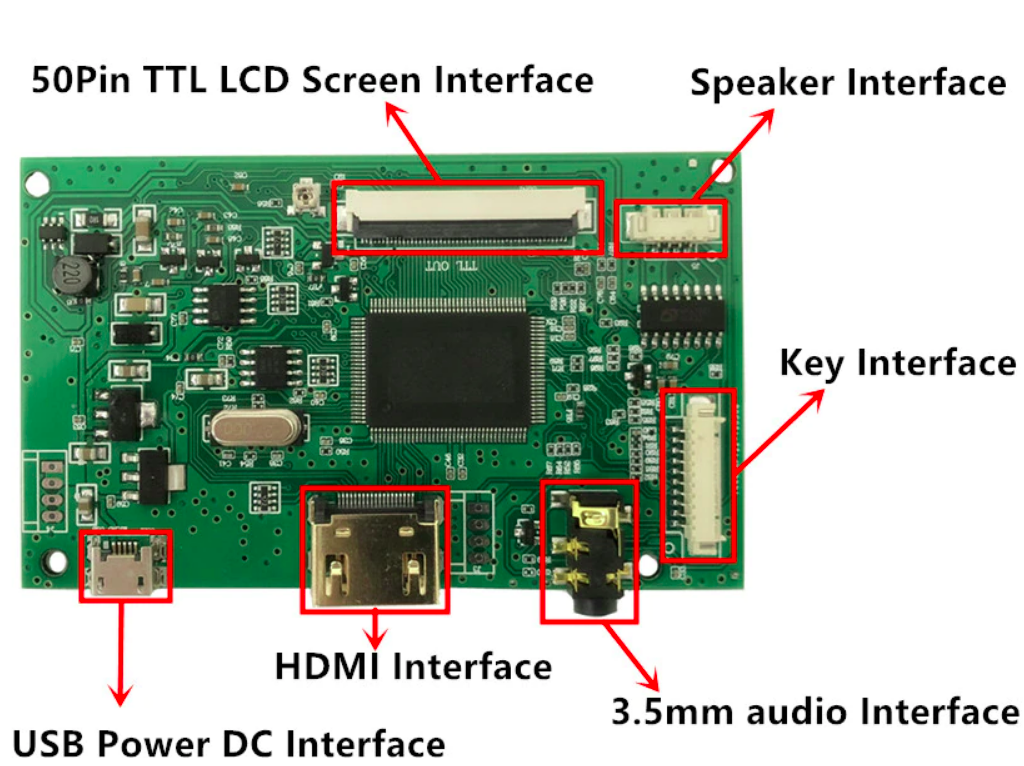
\includegraphics[width=0.6\columnwidth]{./img/screen-interfaces.png}
  \caption{Display Interfaces (withdrawn from \cite{screen})}%
\label{fig:screen-interfaces}
\end{figure}

It can also be seen in this figure that the display has also a remote and a board to handle the remote controls, but in this implementation, it will probably not be in use.

\subsection{Speakers}
When playing video ads, it is not only necessary a display, but also a speaker to playback the sound of the ads.
As it can be seen in Fig.~\ref{fig:screen-interfaces}, the screen board has two different interfaces of audio: the speaker interface and the audio interface.
For this project it will be used speakers that uses the speaker interface, because that type of speakers with that interface are passive speakers and don't need a \gls{dc} power supply, which is an advantage~\cite{passive-speaker}.

Thus, the speakers that will be used have an impedance of \texttt{8 Ohm} and a power of \texttt{5 Watts} and are displayed on Fig~\ref{fig:speakers}.
%
\begin{figure}[htb!]
\centering
    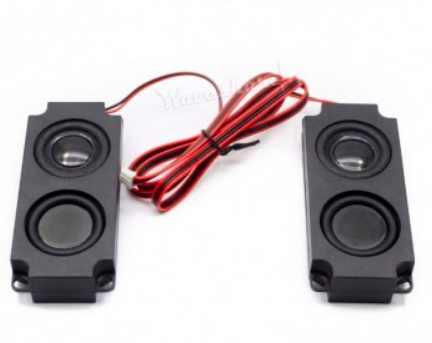
\includegraphics[width=0.4\columnwidth]{./img/speakers.png}
  \caption{Speakers (withdrawn from \cite{speakers})}%
\label{fig:speakers}
\end{figure}

\subsection{Power Supply}
\label{sec:power-supply}
The \gls{mdo-l} will be a plugged in system, so it will be needed a plugged in power supply to supply all the components of the system. In total, the power consumption will not overtake 20 Watts and all the supplies necessary are plugged by USB (Raspberry Pi, Fragrance Diffusion Actuator, and screen). So, it will be used the power supply in Fig.~\ref{fig:power-supply}, that has 4 outputs of \texttt{5 V \gls{dc}} and \texttt{2.4 A \gls{dc}} each.
%
\begin{figure}[htb!]
\centering
    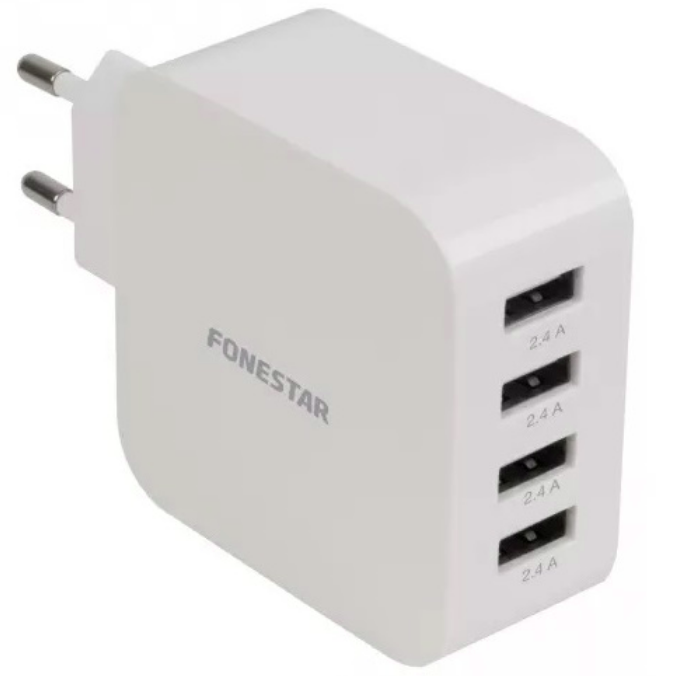
\includegraphics[width=0.3\columnwidth]{./img/power-supply.png}
  \caption{Power Supply (withdrawn from \cite{power-supply})}%
\label{fig:power-supply}
\end{figure}

\subsection{On/Off button}
In this context, an On/Off button can be useful to power On/Off the \gls{mdo-l}. However, this feature is not that necessary, so, this prototype will be only powered through the power supply previously talked in section \ref{sec:power-supply} and will be always on until the power supply be unplugged, powering off the machine.


\subsection{Total \gls{hw} cost}

The total \gls{hw} cost can now be precisely calculated, once that all the
hardware is now specified on table \ref{tab:hw-costs}, yielding about 175 EUR.

% Please add the following required packages to your document preamble:
\begingroup
\renewcommand{\arraystretch}{0.7} % Default value: 1
\begin{table}[!hbt]
% Please add the following required packages to your document preamble:
% \usepackage{booktabs}
\centering
\caption{Total spending on Hardware}
\label{tab:hw-costs}
\begin{tabular}{@{}lrr@{}}
\toprule
\textbf{Item}                & \multicolumn{1}{l}{\textbf{Quantity}} & \multicolumn{1}{l}{\textbf{Price (€)}} \\ \midrule
Raspberry Pi 4B              & 1                                     & 70.00                                  \\ \midrule
Ultrasonic Sensor HC-SR04    & 3                                     & 11.70                                  \\ \midrule
Fragrance Diffusion Actuator & 1                                     & 3.23                                   \\ \midrule
Raspberry Pi Camera V2       & 1                                     & 20.00                                  \\ \midrule
LCD Display                  & 1                                     & 51.95                                  \\ \midrule
Speakers                     & 1                                     & 3.00                                   \\ \midrule
Power Supply                 & 1                                     & 13.50                                  \\ \midrule
\multicolumn{2}{r}{\textbf{Total}}                                   & \textbf{173.38}                        \\ \bottomrule
\end{tabular}
\end{table}

% %  
\section{Hardware interfaces definition}
\label{sec:hw-interf-def}
After specifying the \gls{hw}, it is important to define its interfaces.
Firstly, it is necessary to have basic know-how of the main board's pinout.
In Fig.~\ref{fig:raspberry-pinout} is represented the pinout of the Raspberry Pi.
%
\begin{figure}[htb!]
\centering
    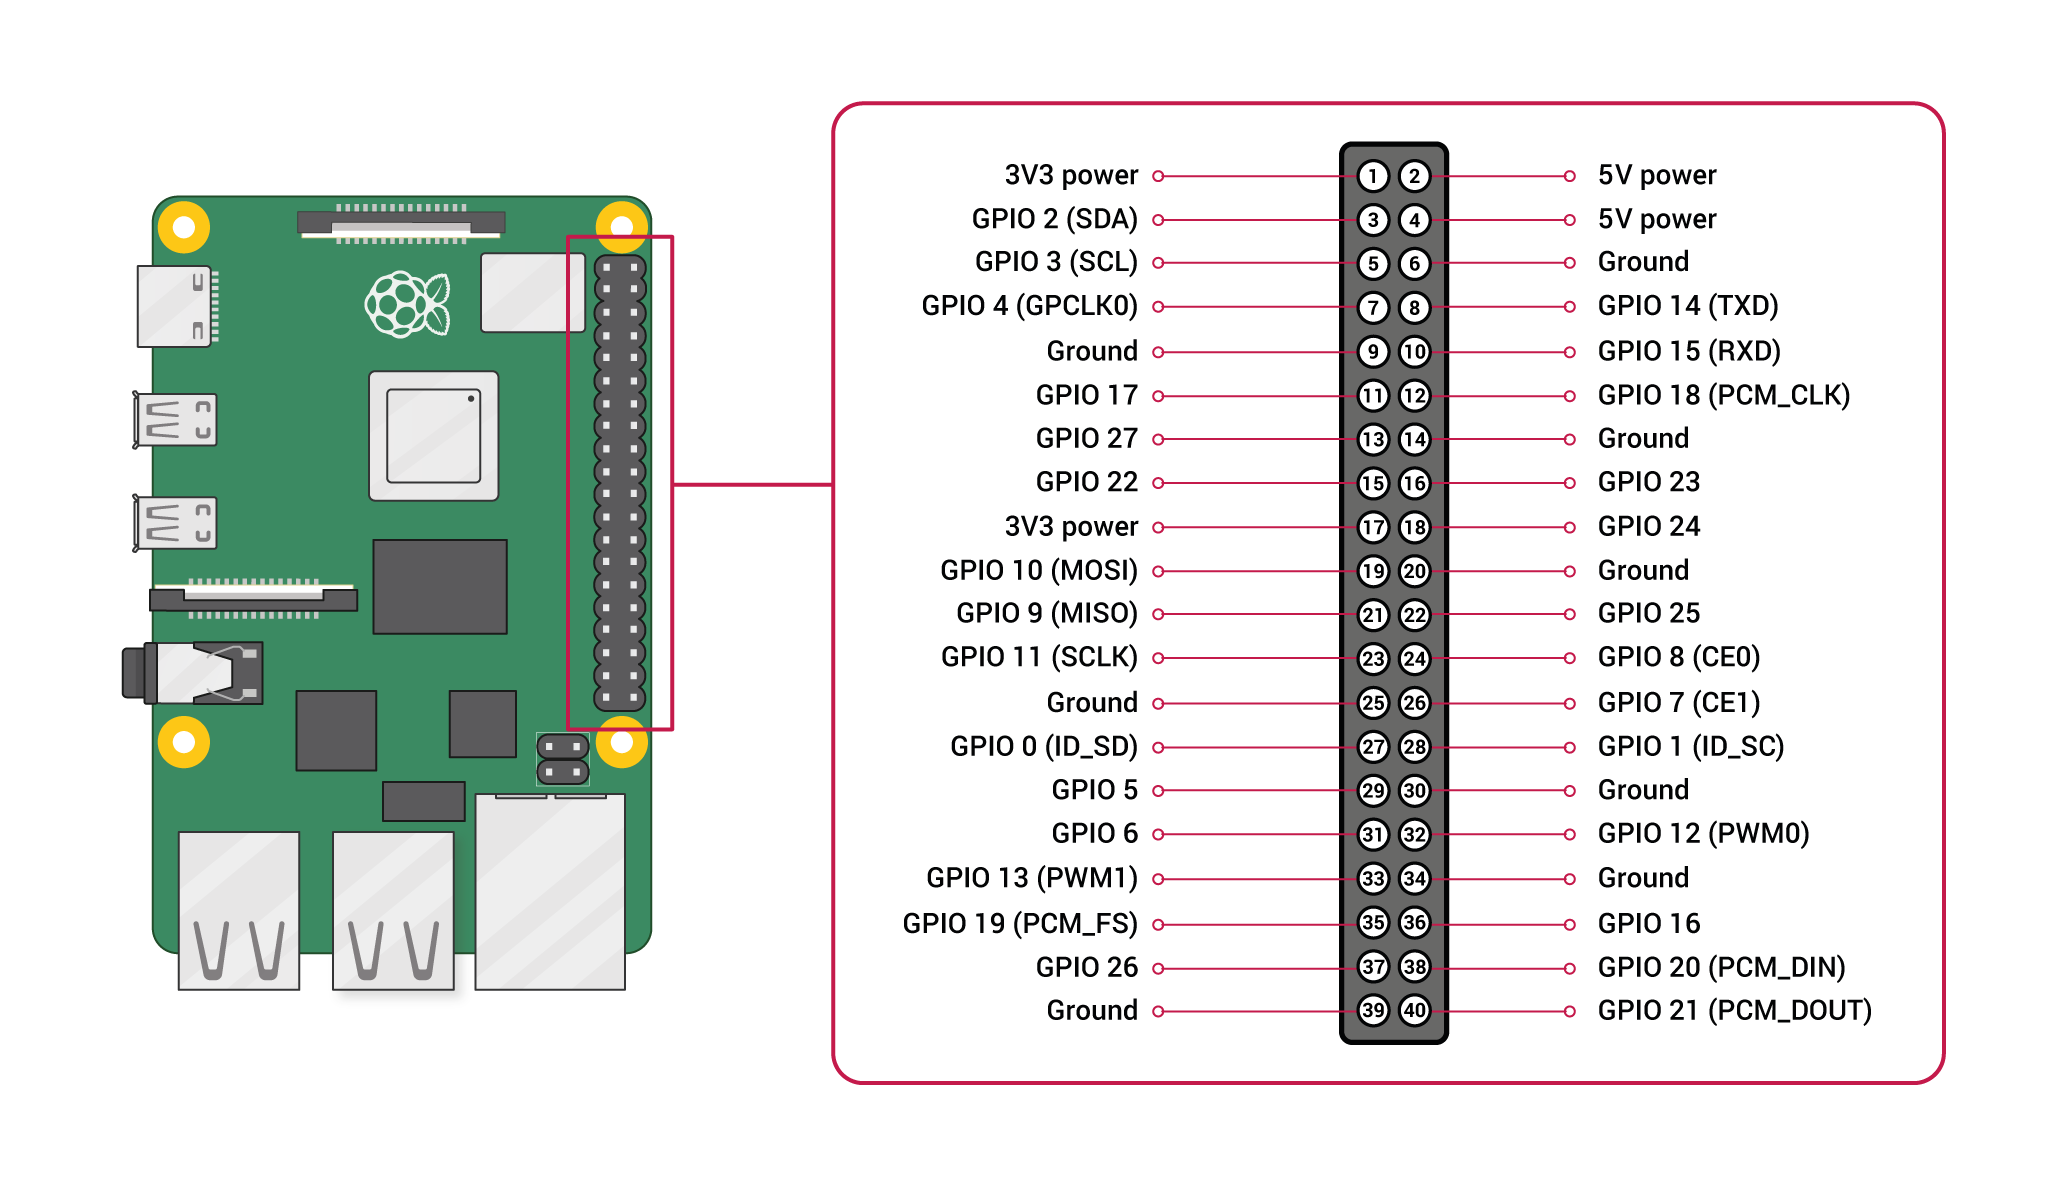
\includegraphics[width=0.9\columnwidth]{./img/raspberry-pinout.png}
  \caption{Power Supply (withdrawn from \cite{raspberry-pinout})}%
\label{fig:raspberry-pinout}
\end{figure}

\subsection{Peripherals Mapping}
\label{sec:periph-map}
After have a basic know-how of the Raspberry's pinout, it is now possible to map all the \gls{hw} components.
As it can be seen in Fig.~\ref{fig:peripheral-mapping}, only two types of peripherals need to be mapped in the Raspberry: the \texttt{ultrasonic sensor} and the \texttt{fragrance diffusion actuator}.

Firstly, the \texttt{ultrasonic sensors} can have three of their four pins in common: the \texttt{Vcc}, the \texttt{GND} and the \texttt{Trig}. The first two are for obvious reasons: they can be powered for the same source, so they are connected to the \texttt{pin 2 (5V power)} and \texttt{pin 9 (Ground)}, respectively. The last one is because the trigger only triggers the sensors to start the acquisition, so, they can all start at the same time and have the same trigger source, so, they are all connected to the \texttt{pin 11 (\gls{gpio} 17)}. Then, each one of them need a specific pin to connect to its \texttt{Echo} in order to make the distance read, so, the pins that are chosen are \texttt{pin 15 (\gls{gpio} 22)}, \texttt{pin 16 (\gls{gpio} 23)} and \texttt{pin 18 (\gls{gpio} 24)}.

Lastly, the \texttt{fragrance diffusion actuator}. Although this one is powered up by Micro-USB, it is necessary to activate or deactivate the diffusion and this is only possible with a \texttt{\gls{mosfet}}, activating its gate. The gate is connected to the \texttt{pin 36 (\gls{gpio} 16)} and this is the pin responsible to activate or deactivate the fragrance diffusion.
%
\begin{figure}[htb!]
\centering
    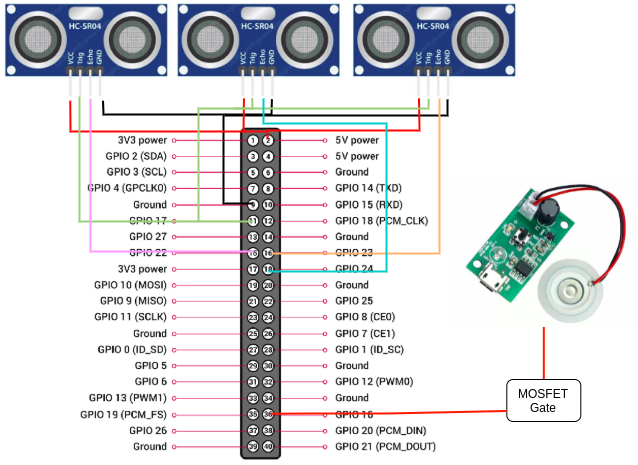
\includegraphics[width=0.8\columnwidth]{./img/hw-pinout.png}
  \caption{Peripheral Mapping}%
\label{fig:peripheral-mapping}
\end{figure}

To turn things more clear, Table~\ref{tab:pin-mapping} shows all the pin mapping in a more clear way.
%
\begingroup
\renewcommand{\arraystretch}{0.7} % Default value: 1
% \useunder{\uline}{\ul}{}
% Please add the following required packages to your document preamble:
% \usepackage{booktabs}
% \usepackage[normalem]{ulem}
% \useunder{\uline}{\ul}{}
\begin{table}[]
\centering
\caption{Pin Mapping}
\label{tab:pin-mapping}
\begin{tabular}{@{}lll@{}}
\toprule
\multicolumn{3}{c}{{\ul \textbf{Pin Mapping}}} \\ \midrule
\textbf{Controller Pin} &
  \textbf{Interface Device Pin} &
  \textbf{Function} \\ \midrule
Pin 2 (5V) &
  Ultrasonic Sensors (Vcc) &
  Supply 5V to the sensors \\ \midrule
Pin 9 (Ground) &
  Ultrasonic Sensors (GND) &
  Close the supply connection \\ \midrule
Pin 11 (GPIO 17) & Ultrasonic Sensors (Trig)  & \begin{tabular}[c]{@{}l@{}}Make pulses to the Trigger's sensors\\ in order to start the distance acquisition\end{tabular} \\ \midrule
Pin 15 (GPIO 22) &
  Ultrasonic Sensor 1 (Echo) &
  \begin{tabular}[c]{@{}l@{}}Handle the Echo Pin of the first sensor\\ in order to measure the distance\end{tabular} \\ \midrule
Pin 16 (GPIO 23) & Ultrasonic Sensor 2 (Echo) & \begin{tabular}[c]{@{}l@{}}Handle the Echo Pin of the second \\ sensor in order to measure the distance\end{tabular}      \\ \midrule
Pin 18 (GPIO 24) &
  Ultrasonic Sensor 3 (Echo) &
  \begin{tabular}[c]{@{}l@{}}Handle the Echo Pin of the third sensor\\ in order to measure the distance\end{tabular} \\ \midrule
Pin 36 (GPIO 16) &
  MOSFET's Gate &
  \begin{tabular}[c]{@{}l@{}}Toggle the gate of the MOSFET in order\\ to turn On/Off the diffusion actuator\end{tabular} \\ \bottomrule
\end{tabular}
\end{table}

\subsection{Test Cases}
\label{sec:test-cases}

In order to verify if all the hardware is in good conditions, are made some test cases to each component.
In Table~\ref{tab:test-cases} are displayed all the test cases to be done in all pieces of \gls{hw}. Basically, all tests are functional tests and need to be done to know if some component may be damaged or also could not be in the error range provided by the manufacturer.
%
% Please add the following required packages to your document preamble:
\begingroup
\renewcommand{\arraystretch}{0.7} % Default value: 1
% Please add the following required packages to your document preamble:
% \usepackage{booktabs}
\begin{table}[]
\centering
\caption{Hardware Test Cases}
\label{tab:test-cases}
\begin{tabular}{@{}llll@{}}
\toprule
\textbf{HW Component} &
  \textbf{Type of test} &
  \textbf{Description} &
  \textbf{Expected Result} \\ \midrule
\begin{tabular}[c]{@{}l@{}}Ultrasonic \\ Sensor\end{tabular} &
  Functional &
  \begin{tabular}[c]{@{}l@{}}One will connect the ultrasonic sensor\\ to the Raspberry Pi. Then, an object\\ will be approximated to the sensor \\ from several distances with the\\ corresponding distance being measured\\ with a  measuring tape.\end{tabular} &
  \begin{tabular}[c]{@{}l@{}}If the distance measured by the \\ sensor and the measuring device \\ are within the error margin \\ provided by the manufacturer,\\ the device is compliant.\end{tabular} \\ \midrule
Camera &
  Functional &
  \begin{tabular}[c]{@{}l@{}}One will connect the camera to the \\ Raspberry Pi and then will try to make \\ image acquisition in real time, take \\ pictures and also try to take some gifs \\ and videos.\end{tabular} &
  \begin{tabular}[c]{@{}l@{}}If the quality of the image and the \\ image  acquisition are in good \\ quality according to the \\ manufacturer's information, then \\ the device is in good conditions \\ of use.\end{tabular} \\ \midrule
\begin{tabular}[c]{@{}l@{}}Fragrance \\ Diffusion\\ Actuator\end{tabular} &
  Functional &
  \begin{tabular}[c]{@{}l@{}}One will connect a MOSFET to the \\ fragrance diffusion and connect its \\ gate to the Raspberry Pi. Then, one \\ will trigger the MOSFET's gate and \\ watch the actuator's behavior.\end{tabular} &
  \begin{tabular}[c]{@{}l@{}}If the diffusion actuator diffuses \\ in good state the fragrance and \\ also if the MOSFET  doesn't \\ overheat, then the set of HW is \\ in good conditions of use.\end{tabular} \\ \midrule
Power Supply &
  Functional &
  \begin{tabular}[c]{@{}l@{}}One will connect the three components\\  (LCD, Fragrance Diffusion Actuator \\ and Raspberry Pi) to the power supply \\ and see their behavior.\end{tabular} &
  \begin{tabular}[c]{@{}l@{}}If all components work properly, \\ then this  piece of HW is in good \\ conditions of use.\end{tabular} \\ \midrule
Speakers &
  Functional &
  \begin{tabular}[c]{@{}l@{}}One will connect the Speakers to the \\ LCD board and try to run a video with \\ sound in order to verify the sound \\ provided by the speakers.\end{tabular} &
  \begin{tabular}[c]{@{}l@{}}If the sound output matches\\ the manufacturer's \\ characteristics of the product, \\ then this set of HW is compliant.\end{tabular} \\ \midrule
LCD Display &
  Functional &
  \begin{tabular}[c]{@{}l@{}}One will connect the LCD board through\\  HDMI to the Raspberry Pi, the LCD \\ Display to its board and supply the board \\ and then try to send some images and \\ videos to the LCD Display.\end{tabular} &
  \begin{tabular}[c]{@{}l@{}}If the images and videos are \\ displayed in good quality and are \\ in match with the manufacturer's \\ information, then this set of HW \\ is in good conditions of use.\end{tabular} \\ \bottomrule
\end{tabular}
\end{table}
%  
%%% Local Variables:
%%% mode: latex
%%% TeX-master: "../../../dissertation"
%%% End:
